\chapter{Literature review}
\label{LR}

\section{Methods of Modelling Phages and Bacteria}
There are numerous ways to model the interactions between phages and bacteria.
Models can be built at a molecular level, where the model simulates the mechanical and chemical behavior of a phage as it interacts with the surface of a bacterium using computational chemistry methods.
On the other end of the spectrum, a different type of model can be built where populations of phages, bacteria, and resources can be modeled using Ordinary Differential Equations (ODEs) or Delay Differential Equations (DDEs).
DDEs are similar to ODEs, except where when ODEs are calculating the values of the equations at time $t$ using time $t-1$, DDEs can, but don't have to, use the value of the equation at time $t-\tau$, where $1 \leq \tau \leq t$. 
DDEs are a generalized version of ODEs and are significantly harder to analyze and find stability conditions than ODEs due to the dependence on the past \cite{liExploringComplicatedBehaviors2023}. \newline
One way to introduce DDE like behavior is to force agents to go through stages, causing a delay in other events. 
For example, in the paper \citet{gengUsingBacterialPopulation2024}, infected bacteria go through $M$ stages of infection, before lysing. 
The more stages there are, the longer the delay in seeing a rise in phage population. By changing the value of $\tau$ in the model proposed by \citet{gengUsingBacterialPopulation2024}, the throughput of bacteria going from stage $i$ to stage $i+1$ of infection increases, thus seeing a larger rise in phage population. 

Each type of model has its pros and cons.
With the molecular level model, the model is more complex and needs significantly more startup time, simulation time, and is in general much more complex.
However, more information can be gained from the simulations and can guide research in creating phages for a certain type of bacteria.
The ODE method is simpler and easier to set up, however it can only capture large population dynamics.
Certain assumptions about the community interactions have to be made.
For example, $\omega$ percent of the bacteria population is washed out.
The model can be made more complicated, by modelling each stage of the phage replication and lysis process, or instead of assuming exponential growth, there is a maximum carrying capacity of the population.
The model can be further altered by using a normally distributed variable $\textbf{N}(\mu=\omega, \sigma=1)$ to account for noise when measuring the data. 
Ensuring the use of a seed value will ensure that each run of the model results in the same output. 

\subsection{Generalized Lotka-Volterra Model}
The Lotka-Volterra model, a first-order non-linear differential model, captures the dynamics between predators and prey.
Any population can be modelled as such:
\[ 
    \frac{d{B}_i}{dt} = {B}_i \left(\left(r_i + \sum_{j}^{N} \alpha_{ij}{B}_j \right) - m_i\right)
\]
where $r_i$ is reproduction rate, $\alpha_{ij}$ is the devour rate of $B_i$ on $B_j$. If $\alpha_{ij}$ is negative, then $B_i$ has a negative effect on $B_j$, otherwise $B_i$ has a positive effect on $B_j$. $m_i$ is the removal rate of $B_i$. 
The interactions can be seen in \Cref{fig:lotka_volterra_model}
 
\subsection{Generalized Consumer-Resource Model}
The generalized Consumer-Resource Model models the growth of a population and resource dynamics between a population of bacteria ${B}_i$ and a resource ${R}_i$. 
\begin{align}
    \frac{d{B}_i}{dt} &= r_i{B}_i \left(\sum_{\alpha} \Delta w_{i \alpha}C_{i \alpha}R_{\alpha}\right) - m_i {B}_i \label{eq:generalized_consumer_resource_model_1}\\
    \frac{dR_{\beta}}{dt} &= -\sum_i C_{i\beta}R_{\beta}{B_i} + \sum_{\alpha, i}D_{\beta\alpha}^{i}C_{i\alpha}R_{\beta}{B}_i \label{eq:generalized_consumer_resource_model_2}\\
    \Delta w_{i\alpha} &= \sum_{\beta}D_{\beta \alpha}^{i}w_{\beta} \nonumber
\end{align}
\Cref{eq:generalized_consumer_resource_model_1} describes the growth of population $B_i$ and \Cref{eq:generalized_consumer_resource_model_2} describes the resource dynamics and metabolism of resource $R_\beta$. 
Resource $R_\alpha$ can become resource $R_\beta$ at rate $R_{\beta \alpha}^{i}$. 
Bacteria $B_i$ reproduces at rate $r_i$ dependent on the concentration of resources $\sum_\alpha C_{i\alpha}$. 
Bacteria die out at rate $m_i$. 
For a visual, see \Cref{fig:consumer_resource_model}


\subsection{Trait-Based Model}
The Trait-Based Model is a model that takes into account external factors such as the temperature or pH of the system and can be modeled as follows. 
\begin{align*}
    \frac{dB_i}{dt} &= \left(r_i - m_i\right) B_i \\
    r_i &= \frac{r_{i\alpha}^{max}R_\alpha}{R_\alpha + K_{i\alpha}}e^{S_i\left(T-T_{ref_i}\right)}
\end{align*}
where $r_i$ is influenced by the environment impact factor. $S_i$ is the sensitivity to $B_i$ to factor $T$, and with trade off if $r_i^{max} > \text{ mean } r^{max} \text{ then } S_i > \text{ mean } S$. 
The larger $S1_i$ is, and the larger the difference $T$ is from $T_{ref_i}$, the stronger the effect will have on the growth rate of $r_i$. 
$r_i$ follows the Monod equation, with $r_{i\alpha}^{max}$ being the maximum growth rate of bacteria $B_i$, $R_\alpha$ is the resource concentration, and $K_{i\alpha}$ is the affinity constant. 
\Cref{fig:trait_based_model} shows the agent interactions in detail. 

\subsection{Agent-Based Models}
ABMs model the system through space and time.
An $x \times y$ grid is created and split into smaller sub-cells containing resources and microbes.
Each cell acts as its own tiny environment, where resources and microbes interact within the cell, but not with the neighboring cells.
Resources diffuse through the system using a PDE solver for a Boundary Value Problem (BVP).
Agents can move into neighboring grids with a probability $p$, where $p$ can depend on any number of parameters such as resource density, microbe density, or stochastic chance. \newline 
ABMs are useful when simulating many individual elements interacting in a system.
Chaotic or emergent behavior can arise from these interactions.
Chaotic behavior refers to the irregular and unpredictable evolution of a system's behavior due to nonlinear equations, exhibiting sensitive dependence on the initial condition (IC) \cite{encyclopedia_of_physical_science_and_technology}. \newline 
Emergent behavior is behavior that arises from the interactions of various agents in a system, that was not explicitly programmed into the system.
The behavior can be beneficial, neutral, or harmful, but it can not be predicted until it arises, \textit{if} it arises.
Agents can have simple rules, but when interacting with other agents, behavior that hasn't been programmed can arise.
Sometimes, people consider systems with emergent behaviors more complex than the sum of their parts. \newline
\begin{align} 
    \label{eq:resource_diffusion}
    \frac{\delta R_\alpha(\left(x, y\right), t)}{\delta t} = \nabla \left[D \left( R_\alpha, \left(x, y\right) \right) \nabla R_\alpha \left(\left(x, y\right), t \right) \right]
\end{align}
\Cref{eq:resource_diffusion} describes the diffusion of resource $R_\alpha$ through the matrix cells, dependent on the resource concentration $R_\alpha$ at cell location $(x, y)$. 
The rules for cellular agents follow \Cref{eq:agent_rules}. 
\begin{align} 
    \label{eq:agent_rules}
    \frac{di}{dt} = r_i \left( \sum_\alpha \Delta w_{i\alpha}C_{i\alpha}R_\alpha\right)
\end{align}, 
where $i$ is a bacterial agent, where if $0 \leq \text{ threshold } \leq \frac{di}{dt} \leq 1$, some threshold, $\frac{\frac{di}{dt}}{2}$ expands into the neighboring grid cell with probability $p$. 
Agent $i$ consumes resources and converts them into new resource with \Cref{eq:agent_consumption_and_conversion}. 
\begin{align} 
    \label{eq:agent_consumption_and_conversion}
    \frac{dR_\beta}{dt} &= \sum_i C_{i\beta}R_\beta I + \sum_{\alpha, i}D_{\beta \alpha}^{i} C_{i \alpha} R_\alpha i
\end{align}
\Cref{fig:agent_based_model} shows how the agents interact with other agents in their cell. 

\begin{figure}[h!]
    \centering
    \begin{subfigure}{0.49\linewidth}
        \centering
        \captionsetup{width=1\linewidth}
        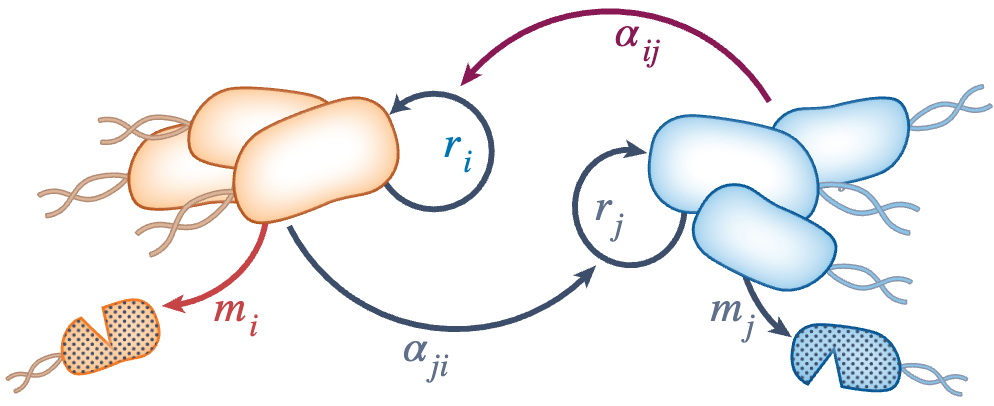
\includegraphics[width=\linewidth]{Figures/lotka_volterra_model.png}
        \caption{
            Lotka Volterra model.
        }
        \label{fig:lotka_volterra_model}
    \end{subfigure}
    \hfill
    \begin{subfigure}{0.49\linewidth}
        \centering
        \captionsetup{width=1\linewidth}
        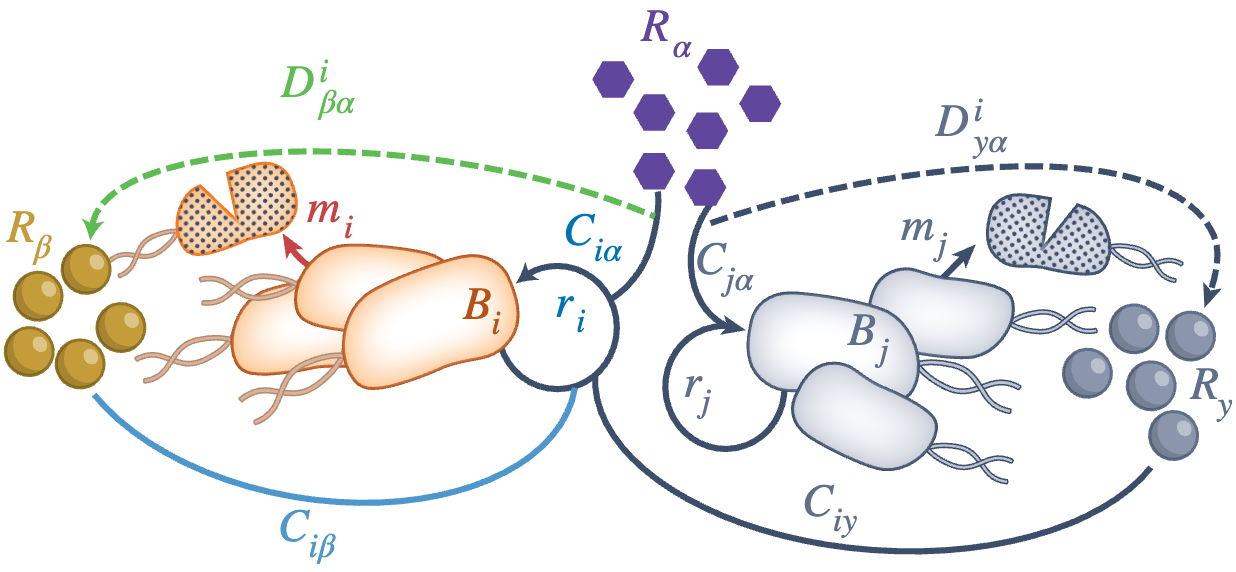
\includegraphics[width=\linewidth]{Figures/consumer_resource_model.png}
        \caption{
            Consumer Resource model.
        }
        \label{fig:consumer_resource_model}
    \end{subfigure}
    \hfill
    \begin{subfigure}{0.49\linewidth}
        \centering
        \captionsetup{width=1\linewidth}
        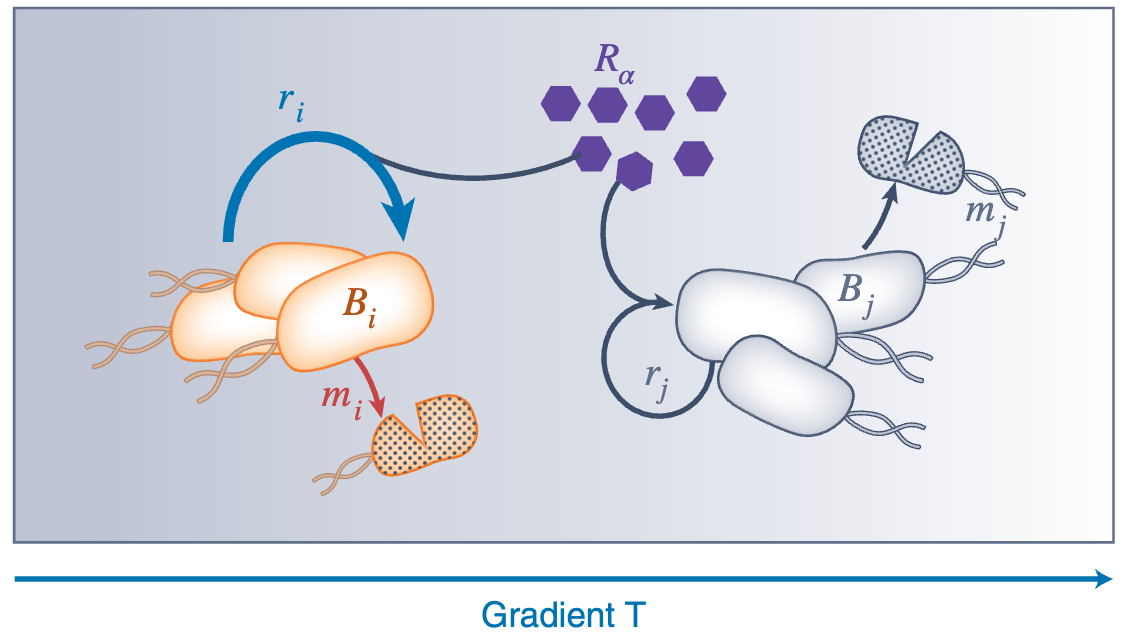
\includegraphics[width=\linewidth]{Figures/trait_based_model.png}
        \caption{
            Trait Based model. 
        }
        \label{fig:trait_based_model}
    \end{subfigure}
    \hfill
    \begin{subfigure}{0.49\linewidth}
        \centering
        \captionsetup{width=1\linewidth}
        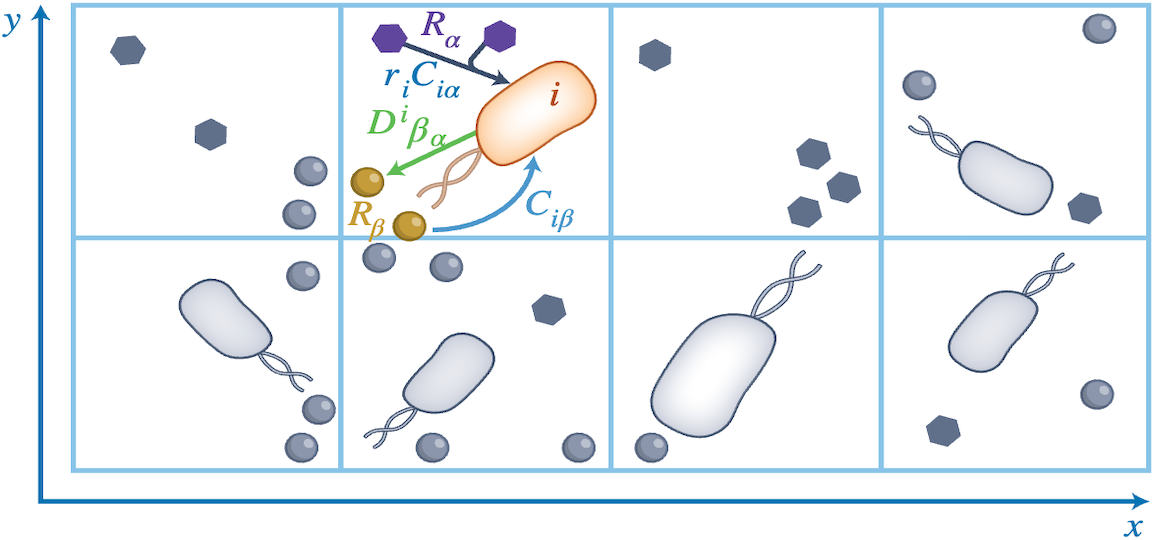
\includegraphics[width=\linewidth]{Figures/agent_based_model.png}
        \caption{
            Agent Based model. 
        }
        \label{fig:agent_based_model}
    \end{subfigure}
    \caption{Different models and how the bacterial agents interact with itself, one another, resources and the environment. All figures sourced from \citet{vandenbergEcologicalModellingApproaches2022}}
\end{figure}


\section{Phage Biology}
\subsection{What Are Phages?}
Phages are small bundles of proteins that contain viral DNA. 
Phages are made up of multiple parts built like LEGO to complete the task of infecting a bacterium. 
\Cref{fig:figures:phage_diagram} shows the body parts of a phage. 
The aim of the phage is to find a suitable bacterial host and infect the host with viral DNA. 
The DNA alters the host's metabolic pathways to its benefit and hijacks the cellular replication process to create new copies of the phage. 
Eventually, the cell lyses, releasing the newly created phages into the environment to infect more bacteria. 
\begin{figure}[h!]
    \centering
    \begin{subfigure}{0.25\linewidth}
        \centering
        \captionsetup{width=1\linewidth}
        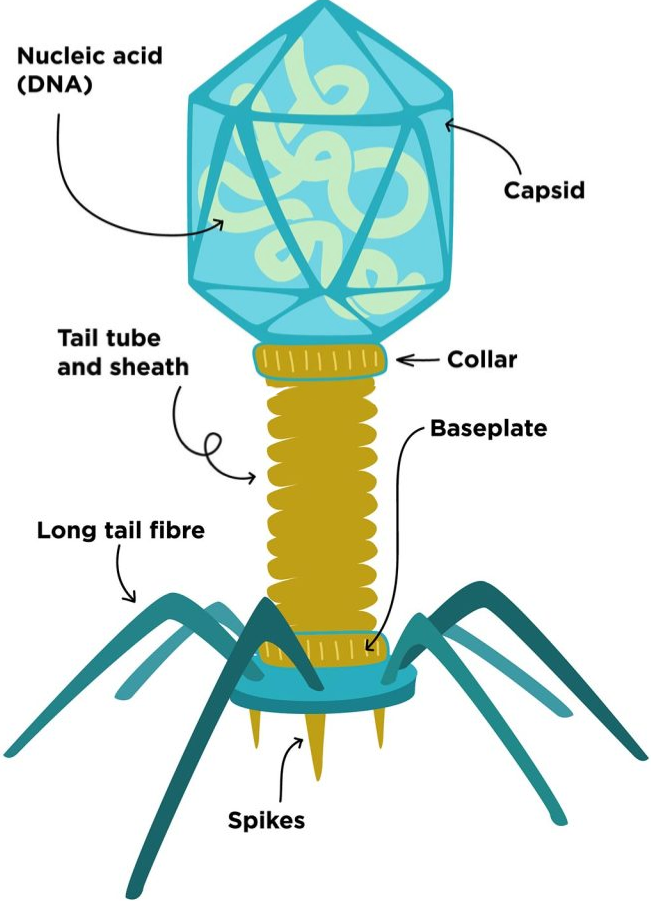
\includegraphics[width=\linewidth]{Figures/phage_diagram.png}
        \caption{
            Phage body structure. 
            % (https://www.newyorker.com/tech/annals-of-technology/phage-killer-viral-dark-matter). 
        }
        \label{fig:figures:phage_diagram}
    \end{subfigure}
    \hfill
    \begin{subfigure}{0.3\linewidth}
        \centering
        \captionsetup{width=1\linewidth}
        \includegraphics[width=\linewidth]{Figures/phage_real.png}
        \caption{
            Phages infecting an \textit{E. coli} bacteria. 
            % (https://www.newyorker.com/tech/annals-of-technology/phage-killer-viral-dark-matter). 
        }
        \label{fig:figures:phage_real}
    \end{subfigure}
    \hfill
    \begin{subfigure}{0.35\linewidth}
        \centering
        \captionsetup{width=1\linewidth}
        \includegraphics[width=\linewidth]{Figures/phage_impression.png}
        \caption{
            Artist representation of phages infecting a bacterium. 
            %(https://www.gettyimages.nl/detail/foto/bacteriophage-virus-attacking-a-bacterium-royalty-free-beeld/1179038792). 
        }
        \label{fig:figures:phage_impression}
    \end{subfigure}
    \caption{Parts of a phage, a real life picture of phages infecting an \textit{E. coli} bacterium, and an artist's impression of phages infecting a bacterium. }
\end{figure}

\subsection{How Does the Phage Cycle Work?}
There are 3 main parts to the phage-bacteria host cycle, the infection stage, the lysogenic cycle, and the lytic cycle. 
In the infection stage, a phage floating through the environment detects and attaches to the surface of a bacteria cell. 
Once injected, the phage-cell pair can directly go into the lysogenic cycle or into the lytic cycle. 
\Cref{fig:phage_life_cycle} shows a detailed overview of the phage cycle. 
\newline 

In the lysogenic cycle, the phage DNA injects integrates into the genome of the bacteria. 
As the bacteria undergoes cellular replication, the DNA of the phage will be copied with the cell. 
After a set amount of time, the phage DNA can cut itself from the genome and enters the lytic cycle.
\newline 

In the lytic cycle, the phage hijacks the cellular process of the bacteria. 
The phage DNA hijacks the replication, transcription, and replication process of the cell, making more and more copies of phage. 
The phage parts build together to make a full part. 
Eventually the cell wall bursts releasing the phages into the environment ready to infect more bacteria. 

\subsubsection{Infection Stage}
The infection stage is characterized as the searching for a bacterium, detection, and subsequent attachment and injection of DNA into the bacteria. 
\paragraph{Detection and Attachment}
Phages float through the medium and by chance land on a bacteria. The phage detects the cell via phage receptor binding proteins located at the tip of the phage tail. 
Various inter-molecular forces such as hydrogen bonds help the phage detect and attach to the cell. 
The receptors are tuned to specific receptors found on the surface of the bacteria cell wall. 
Upon detection, conformational alterations in the phage's baseplate occur, causing changes in protein shapes, causing the sheath to contract and inject the viral DNA into the host. 
The successful binding and adsorption depends on the phage binding protein sensitivity, localization,and density of receptors. \cite{stoneUnderstandingExploitingPhage2019}. 
\paragraph{Phage DNA Injection}
The injection is triggered by the recognition between the phage's receptor-binding protein located at the tip of the tail and a specific receptor located on the surface of the bacteria. 
Once a suitable injection site has been identified, the phage injects the DNA into the cytoplasm of the cell. 
The specificity of recognition is directly related to the specificity of adsorption, which correlates to the structure of receptors located on the host's cell surface \cite{stoneUnderstandingExploitingPhage2019}. 
The injected DNA is called a plasmid, genetic structure usually in the shape of a circle that can replicate independently of chromosomes. 

\subsubsection{Lysogenic Cycle}
The lysogenic cycle describes the process in which the viral DNA of the phage evades detection, integrates into the cell's DNA, replicates with the cell, and inducts from the DNA. 
Phages that have integrated into the host's DNA are called prophages. 
\paragraph{Repression of DNA}
As phages are viruses, they need to evade viral detection methods such as Cyclic oligonucleotide-based anti-phage signalling systems (CBASS). 
CBASS triggers effector proteins that cause cell death, preventing phage replication and lysis \cite{banhBacterialCGASSenses2023}. 
Two big benefits of programmed cell death is that the cell death slows the growth of phages and the dead cells release resources into the environment, allowing other bacteria to recycle the resources and grow \cite{warwick-dugdaleHosthijackingPlanktonicPiracy2019}. \newline
CRISPR-Cas is another method that bacteria can use to detect the presence of phage DNA. 
CRISPR-Cas is an adaptive immune system in bacteria that defends against phages by acquiring foreign DNA sequences (spacers) into its CRISPR array, transcribing them into CRISPR RNAs (crRNAs), and using these crRNAs with Cas proteins to identify and degrade foreign DNA \cite{levyCRISPRAdaptationBiases2015}. 
\paragraph{Phage DNA Integration Into Bacteria DNA}
The DNA of the phage is able to integrate into the bacteria's DNA. 
Prophages can alter the fitness of the cell, by changing metabolic routes and other cellular structures and functions to better survive under resource limitations or by increasing resistance against other phages. 
By altering the fitness of the cell, the prophage can wait until better conditions are met for a lytic approach to be favorable \cite{warwick-dugdaleHosthijackingPlanktonicPiracy2019}. 
\paragraph{Cellular Replication}
The cell undergoes division multiple times, copying the prophage DNA into the cell copies. 
However prophages are still at risk of being discovered and excised by restriction enzymes \cite{sharpMolecularEvolutionBacteriophages1986}. 
\paragraph{Phage Induction}
Prophages induct (leave) from the bacteria DNA under specific conditions. 
The induction process starts with proteolytic cleavage and displacement of the phage repressor, which most of the time occurs upon activation of the SOS response following DNA damage \cite{waldorPhageRegulatoryCircuits2005}. 
Cell stressors such as DNA-damaging agents like UV light and antibiotics can jump-start the process to switch to the lytic cycle \cite{stoneUnderstandingExploitingPhage2019, fortierImportanceProphagesEvolution2013}. 

\subsubsection{Lytic Cycle}
The lytic cycle describes the process in which the viral DNA hijacks the DNA replication process, assembles within the cell, and lyses the cell releasing the phages into the environment. 
\paragraph{Hijacking DNA Replication Process}
The phage hijacks the cellular replication process to create the different proteins that make up the phage, like the legs, body, and head. 
Phenotypic reconfiguration of the host is frequently facilitated by auxiliary metabolic genes, which are genes initially sourced from host genomes but preserved and modified within viral genomes to channel energy and resources toward viral replication \cite{warwick-dugdaleHosthijackingPlanktonicPiracy2019}. 
\paragraph{Assembly of Phage Parts}
Phage parts self-assemble by using various protein-protein and protein-nucleic interactions, along with other forms of interactions such as hydrogen bonding and hydrophobic/philic interactions \cite{aksyukBacteriophageAssembly2011}. 
\paragraph{Lysis of the Bacterial Cell}
Internal pressure buildup causes the cell wall to explode, releasing phages, resources, and other organic matter into the environment. 
Genetic material from one bacteria can be transferred to other bacterial cells via phages, driving bacterial evolution. 


\section{Bacterial Defense Against Phages} 
There is a constant battle between phages and bacteria. 
The bacteria don't want to be killed by the phages, so they adapt defenses such as thickening of the cell wall, or once the viral DNA has integrated with the bacteria's DNA, the bacteria will cut the viral DNA out of their DNA using CRISPR and restriction enzymes \cite{iglerPhenotypicFluxRole2022}. 

\subsection{Mutations in Bacterial DNA (Genetic (Co-)Evolution)}
As bacteria cells grow and divide, random point mutations can occur in the DNA. 
These mutations can affect phage defenses, like thickening the cell wall or removing a receptor, making it harder for the phages to detect and  infect the cell. 
Mutations might not always work, or they can have the opposite effect. 
They can be partially effective if full effectiveness requires multiple steps to achieve, which can occasionally fail \cite{lenskiTWOSTEPRESISTANCEESCHERICHIA1984} or the mutation brings a cost to the bacteria cell by losing receptors on the cell wall. 

Bacteria can horizontally transfer DNA to other bacteria on contact. 
There are three primary ways of this happening, which is visualized in \Cref{fig:horizontal_gene_transfer}. 

The first method is via conjugation, where a donor cell donates DNA fragments using a mechanism called the F-factor or plasmid with a pilus. 
The pilus acts as a tunnel between the donor cell and the recipient cell so that DNA can be transferred from the donor cell to the receiver cell. 
This method of sharing DNA can also have the unintended side effect where one bacteria will directly infect another bacteria by transferring phage DNA. 

The second method, called transformation, occurs when a cell takes up released DNA fragments from the environment. 
Once inside the receiver cell, the donor DNA can integrate itself with the receiver DNA. 
There is also the chance that the bacteria picks up viral DNA \cite{chenInsOutsDNA2005}. 

The third method is via transduction. 
When a phage is assembling in the cell just before lysis, the phage can accidentally collect a piece of the host's DNA instead of its own DNA. 
The dying bacterium proceeds to lyse, releasing the phages. 
The phage with the now dead hosts DNA can infect the next bacteria, injecting the DNA strand of the now dead cell into the new host cell. 
The old bacterial DNA will proceed to integrate with the new host cells DNA \cite{tamangHorizontalGeneTransfer2023, kasmanBacteriophages2025}. 

All methods provide a way for the cell to mutate and change the fitness value of the cell.

\begin{figure}[h!]
    \centering
    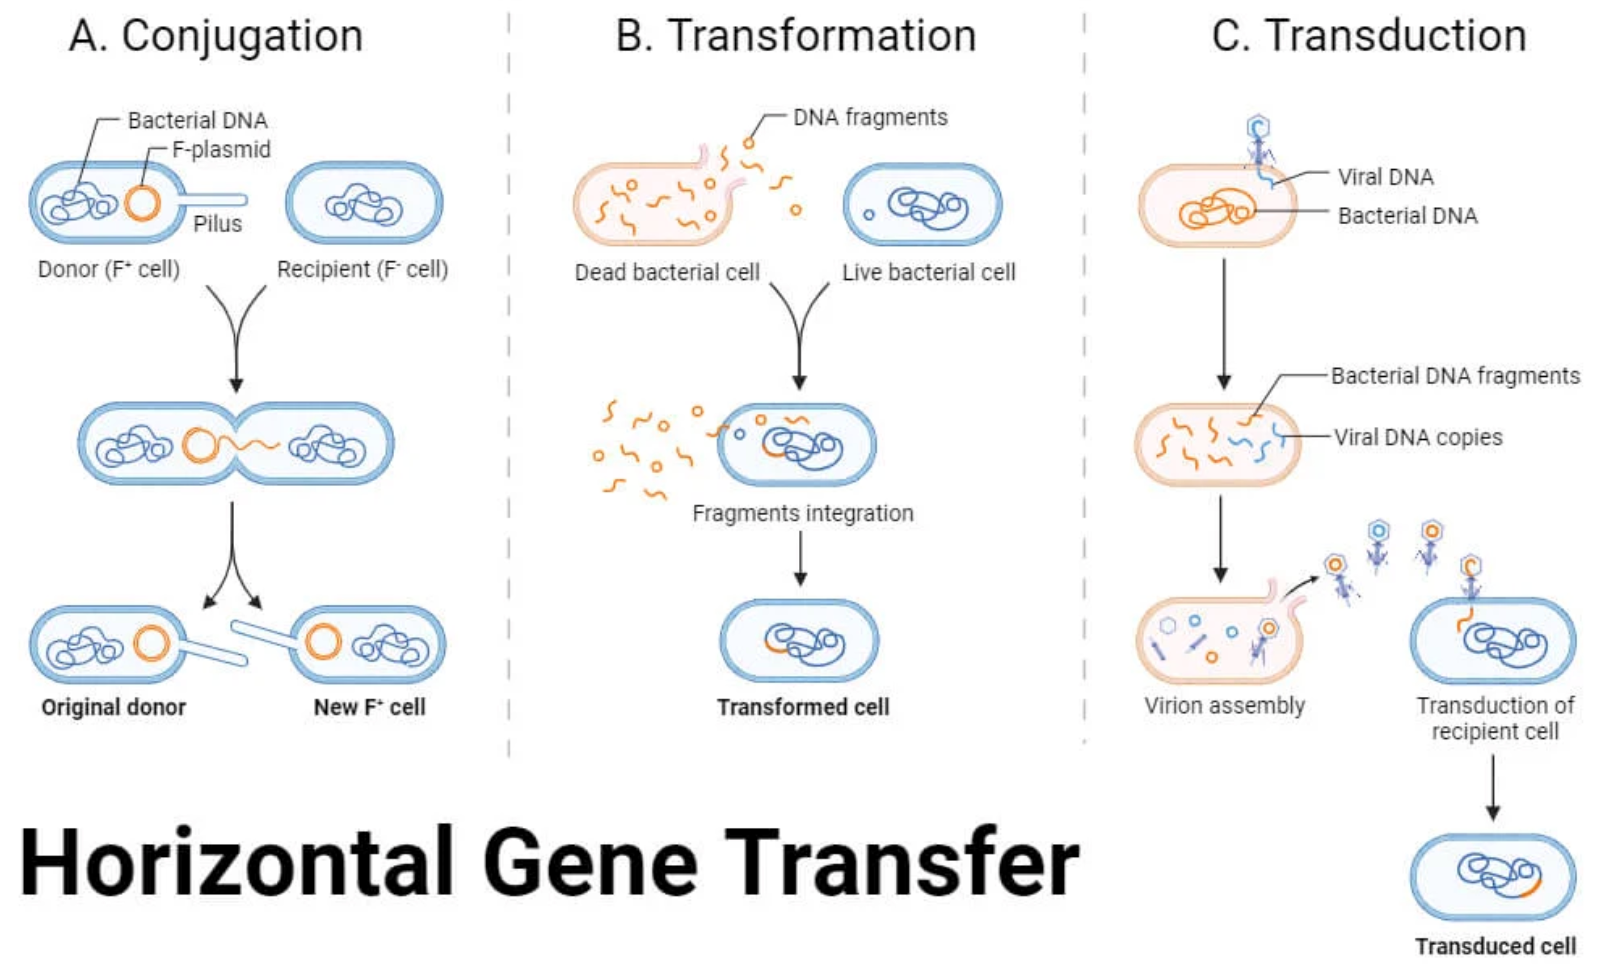
\includegraphics[width=0.7\linewidth]{Figures/horizontal_gene_transfer.png}
    \caption{The three main ways that a (dead) bacterium can horizontally transfer DNA and genes over to another bacterium \cite{tamangHorizontalGeneTransfer2023}.}
    \label{fig:horizontal_gene_transfer}
\end{figure}

\subsection{Phage Inactivation and Decoys}
Bacteria can further protect themselves by producing decoys that the phage will attach to instead of themselves, inactivating the phage. 
Freshly lysed bacteria can still contain biomarkers that phages use to detect the bacteria, but upon injection, nothing happens as the cell doesn't function anymore. 
Bacteria can also produce proteolytic enzymes that will damage the proteins found in a phage \cite{tanQuorumSensingDetermines2015}. \newline
Some bacteria can produce outer membrane vesicles that phages can absorb to, and later detach the vesicle with the phage \cite{rabinovitchBacterialDebrisEcological2003}. 
The vesicle will proceed to float away with the attached phage, posing no risk to itself or to other bacteria. 
It is suspected that the impact of these vesicles acting as a sink is minor \cite{bullPhageBacterialDynamicsSpatial2018}, but helpful nonetheless. 


\subsection{CRISPR-Cas Methods}
CRISPR is a gene editing tool that cells can use to cut out specified/unwanted parts of a DNA strand. 
Researchers are commonly using CRISPR to genetically engineer plants and animals to have specific features. 
Strands of DNA can be selectively added or removed from a DNA strand to achieve a better, more desired DNA strand. 
Specialized defenses in the bacteria can detect unwanted strands and remove the strand, acting as a line of defense against phages. 

\subsection{Phenotype Resistance}
Although mutations can occur in bacterial DNA, not every mutation results in a distinct phenotypic change.
However, there is still a chance that a mutation can change the phenotype representation. 
A mutation can cause the cell wall to thicken, making it harder for a phage to infect the cell. 
The bacterium can decrease the number of receptors that a phage can detect, making it harder for the phage to detect the bacterium. 

\citet{guptaCombinatorialPhenotypicLandscape2025} found that some \textit{Bacteroides fragilis} bacteria were able to evade phage infection.  
The presence of combinatorial phenotypic states where differential expression of protective mechanisms created rare super-resistant cells capable of withstanding phage attack.
By acting together, these heterogeneously expressed anti-phage defense mechanisms created a phenotypic landscape where distinct protective combinations enabled the survival and re-growth of bacteria expressing these phenotypes without acquiring additional mutations. 

\subsection{Spatial Refuge/Biofilms} 
Usually bacteria and phages coexist in well mixed environments such as the ocean, however some environments offer natural structures for bacteria to hide behind. 
These structures can range from physical structure, like sediment in water to biochemical structures like biofilms, where the phages can't diffuse through the biofilm. 
In large enough quantities, bacteria and other microbial communities create biofilms, a layer of mucus containing various microbes. 
The thick mucus, microbes, and other spatial effects help protect the bacteria in the biofilm from external phages by making it hard for the phages to penetrate and diffuse through the mucus \cite{abedonPhageDelayEnhancing2017}. 
In the case of a lab experiment on an agar plate, bacteria protect one another by making it harder for the phages to diffuse through the system \cite{eriksenGrowingMicrocolonyCan2018}. \newline
Phages can not swim and do not contain any parts that allow it to move under its own power. 
Movement is instead passive, relying on the environment to move through the environment, such as diffusion, changes in pressure or heat gradients \cite{lohrmannInfluenceBacterialSwimming2024}. 
The motion that phages exhibit is called Brownian motion, the seemingly random movement of small particles throughout a medium due to other microscopic particles interacting and bouncing off of one another \cite{moineauBacteriophage2013}. 
Unlike phages, bacteria have the ability to actively move through the environment, and they can use this to their advantage by crawling or swimming away if they detect a phage. 

\subsection{Other Methods of Defense}
Other methods of defense include phage restriction by prokaryotic argonaute proteins, production of small molecules that block phage propagation, depletion of molecules essential for phage replication, systems that use small molecule signaling to activate immune effectors, retrons that involve reverse-transcription of non-coding RNAs, and more \cite{stokar-avihailDiscoveryPhageDeterminants2023}.


\section{Phage Counter Defense Against Bacteria}
With some of the defenses that bacteria have developed, phages are always mutating to counter their defenses. 
If phages don't adapt to the ever-changing bacterial defenses, the phages will die out due to their inability to infect and multiply. 
It essentially becomes a race to the bottom, seeing who can out-adapt the other. 
However, if the phages out-adapt the bacteria too much, the bacteria die out, then eventually the phages die out due to not having any bacteria left to infect. \newline
This can be avoided if the phages can adapt to target a second strain of bacteria, but this is unlikely. 
On the other hand, if bacteria out-adapt the phages, that is no problem for the bacteria because they don't need the phages to survive, and can keep on growing, limited only by the available space and resources. 

This is a problem intrinsic to predator-prey systems, namely that the predators are dependent on the prey. 
Once the prey disappear, the predators also disappear. 
If the prey population goes down, and as a result the predator population goes down and becomes extinct, the prey can come back without the threat of predators. 

Phages face this exact same problem: the complete removal of either the bacteria or phages will lead to the removal of the phages from the system unless reintroduced. 

\subsection{Genetic Mutations}
Mutations in viral DNA will affect how the phage body parts are designed and built. 
These mutations will affect external phage behavior such as how it detects a bacteria, as well as internal behavior such as evading detection and integrating with the cell's DNA. 
The changes will lead to changes in overall phage fitness, ie the ability for the phage to infect, replicate, and lyse bacteria. 

\subsection{Viral Recombination}
https://www.sciencedirect.com/science/article/pii/S1931312821004170
https://pmc.ncbi.nlm.nih.gov/articles/PMC3185693/
Multiple phages can infect a cell and replicate itself using the cells internal replication process. 
Each phage has its own building blocks. 
Phage 1 could have long legs, a long neck, and a small head, while phage 2 can have long legs, a long neck, and a medium-sized head. 
When the phages are building copies of themselves, they could accidentally use the body parts of other phages. 
The primary method for proteins to bond with other proteins and molecules is via hydrogen bonds. 
These attractive forces hold proteins and other molecules in defined positions, and a change in molecule shape will change the bonds, which will force the other molecule to undergo changes in shape. 
If the proteins that build the subparts of each phage have similar chemical properties, they can be swapped between phages. 
This allows for biological diversity to spread throughout a phage population. 
Each phage body part can have unique characteristics such as better attachment rate, larger DNA storage capsule, or better probability of injection. 

Coexistence between phages and bacteria via genetic co-evolution seems unlikely due to trade-offs imposed by the new mutations \cite{bullOptimalityModelsPhage2006}. 


\section{Phage Defense Against Phages}
Some phages can employ defenses against other phages from infecting the bacterial cell ensuring the hots resources are all for itself. 
\subsection{Superinfection Exclusion}
The act of preventing a secondary infection form a similar or closely related phage is called superinfection exclusion (SIE). \cite{patelAntiphageDefenceInhibition2024}. 
There are various methods of preventing further infections. 
\subsection{Altering Cell Structure}
The prophage can alter the surface receptors of the bacteria, making it harder for other phages to detect the bacteria, reducing the chance of attachment and injection by other phages \cite{bucherPhageMachineSIEence2024}. The prophage can hijack the internal metabolic pathway and cellular functions, affecting the genes that are expressed and transcribed to proteins. 

\subsection{Protein Creation}
Other phages like the T4 phage can use proteins like the Spackle protein. 
The Spackle protein inhibits the lysozyme activity used in the process of DNA injection by other phages \cite{bucherPhageMachineSIEence2024, kanamaruStructureFunctionT42020}. 
Some prophages can encode proteins that will interfere with the replication process of other phages. 
For example, the SieA protein encoded by phage P22 blocks infection from other phages \cite{leavittBacteriophageP22SieAmediated2024}. \newline
TAB (Tail Assembly Blocker) is an anti-phage defense mechanism encoded by a \textit{Pseudomonas aeruginosa} prophage. 
While TAB permits the invading phage to replicate its genome, it inhibits the assembly of the phage tail, thereby preventing the production of infectious virions. 
The prophage that encodes TAB is not affected by this inhibition, as it also expresses a protein that neutralizes TAB's blocking activity. 
Although the host cell still undergoes lysis, no infectious phages are released.

\subsection{Implications of Phage Against Phage Defense}
SIE can affect the speed and development of phage and bacterial populations. A phage restricting other phages from infecting the bacteria creates a competitive environment and can out-compete and dominate the other population. 
This is commonly seen in wildlife populations, where invading species can out compete other species by consuming resources faster than local species, breeding at a faster rate than other species, and having no natural predators. 

\section{Bacteria and Phages in the Lab}
Researchers around the world are running lab experiments to gain further knowledge of the interactions between phages and bacteria. 
The aim is to better understand how phages work and interact with bacteria at a molecular, host, and population level. 

A researcher might run the experiment in a liquid medium containing water, carbon and nitrogen sources, and other chemicals such as anti-foaming or pH control chemicals. 
This liquid medium, often referred to as broth, allows for the cultivation of bacteria in a well-mixed environment, enabling researchers to monitor bacterial growth and phage infection dynamics over time. 
By adjusting parameters such as nutrient concentration, temperature, agitation speed, and pH, researchers can simulate different environmental conditions and observe their effects on phage-bacteria interactions. 
Samples can be taken at various time points to measure bacterial density, phage titer, and resource depletion, providing quantitative data for model validation and hypothesis testing. 
If measured frequently enough, the researcher can get an ODE-like curve out, where each line shows the population levels at that time. 
Researchers can create a mathematical interpretation of the curves and run algorithms such as curve fitting and simulated annealing to find and tune the ODE model parameters. 
The tuned ODE parameter values tell the researcher the reaction rate speeds, the burst size of the cell, and cell latent period \cite{gengUsingBacterialPopulation2024, mullaExtremeDiversityPhage2024}. 
Chemostats and batch cultures are commonly used setups, with chemostats allowing for continuous input of fresh medium and removal of waste, maintaining steady-state conditions ideal for studying long-term dynamics.

Petri dishes are another commonly used way to grow bacterial colonies. 
Agar, a jelly-like substance derived from seaweed, is commonly used as a solid growth medium in petri dishes. 
It provides a stable surface for bacteria to grow and form visible colonies. 
By adding nutrients and other supplements to the agar, researchers can tailor the medium to support the growth of specific bacterial strains or to test the effects of different environmental conditions. 
When phages are introduced to a bacterial lawn on agar, clear zones called plaques appear where phages have infected and lysed the bacteria, allowing for quantification and observation of phage activity. 
As a cell lyses, it releases phages into the surrounding. 
The phages can diffuse through the system, infecting neighboring cells. 
A small plaque of size 2-3mm can be created, where there are no bacteria. 

Bacteria density can be measured optically using light. 
In the case of liquid cultures, as the bacteria grow and die, the solution will get more cloudy. 
By shining a light through a control vial with no bacteria growth and through a vial with bacteria growth, the change in light refraction and intensity can be measured. 
A researcher might also be interested in using a mass spectrometer to measure the density of phages and nutrients at specific time points. 

With petri dishes, it is harder to measure the bacterial growth. 
Bacteria are usually mixed with phages in a heated liquid agar solution, and poured onto a petri dish. 
It might be possible to scrape the bacteria off of the dish into a liquid to measure the optical density (OD), but the results are not always consistent. 
A computer vision algorithm might be able to quantify the change in color on the petri dish, by comparing the photo of the bacterial lawn with a reference photo with no bacteria growth. 
Or it can compare the area of growth with area of no growth, where phages are present. 
However the results are sensitive to camera settings, such as exposure and sharpness. 
Lighting can have a big factor in the analysis such as if there are shadows from an object over the plate, or if there is residual sunlight entering the room, making the room brighter or darker. 
It would be easier to measure the change in plaque size, assuming the camera and petri dish stay in the same position for every picture. 
\Cref{fig:phage_petri_dish} shows a sample bacterial lawn with phage plaques. 
If one were to zoom in, \Cref{fig:figures:phage_real} shows stained phages infecting a bacterium. 

Measuring OD is inaccurate and can only accurately measure up to an OD of 0.1. Even though using a special spectrophotometer allows consistent results, the results are dependent on the medium, the length of travel through the medium, bacteria size and density. 
THe device and measurements need to be calibrated to ensure proper results. 
Changing methods to using \textit{cells/ml} over OD can be used to directly compare results across experiments, labs, and bacteria colonies \cite{miraEstimatingMicrobialPopulation2022}. 



\begin{figure}[h!]
    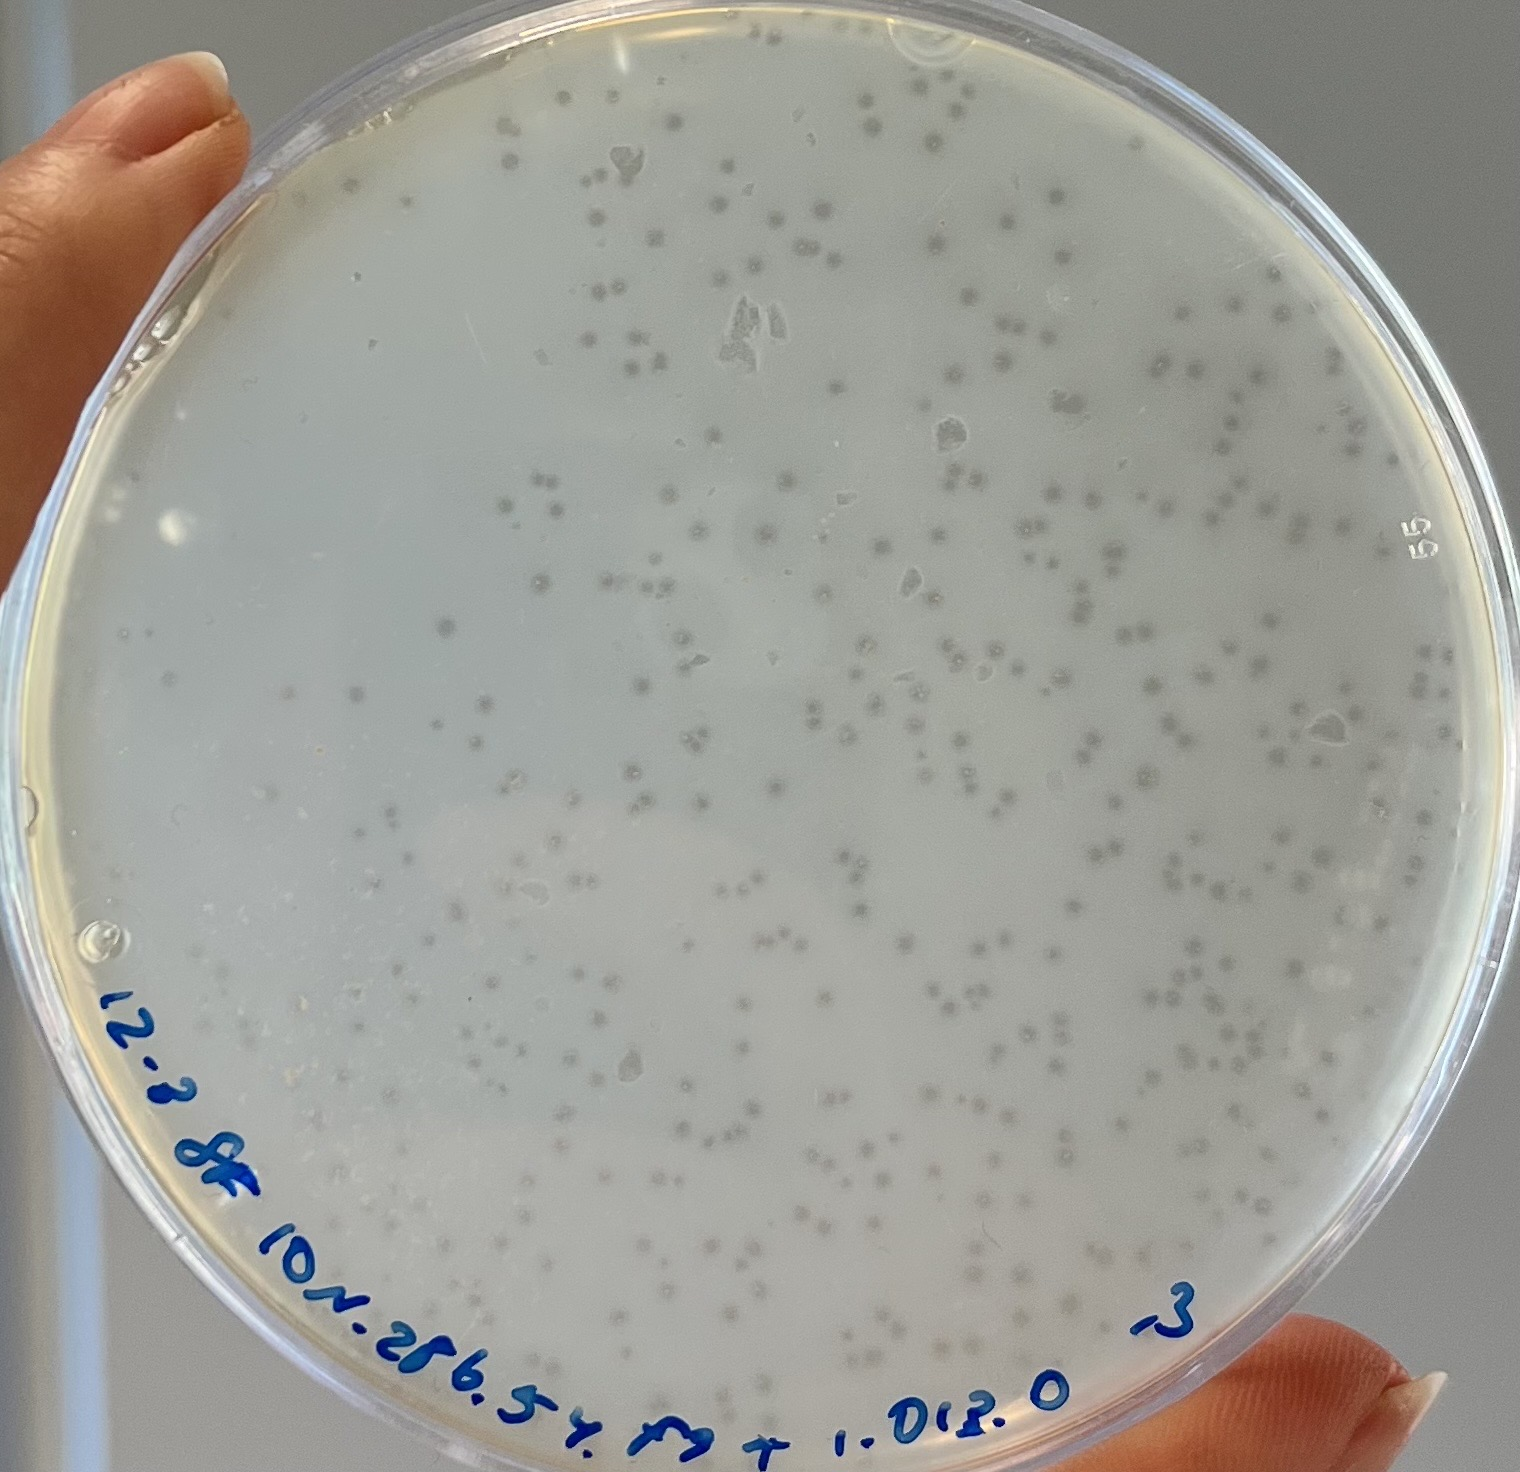
\includegraphics[width=0.7\textwidth]{Figures/phage_petri_dish.jpeg}
    \centering
    \caption{Bacteria lawn, the dots on the petri dish show no bacteria growth due to the presence of phages. Photo courtesy of S. Flickinger. }
    \label{fig:phage_petri_dish}
\end{figure}


\section{Software Mathematically Modelling Phages, Bacteria, and Resources}
Some software programs modelling phage-bacteria-resource interactions already exists. 

\subsection{Cocktail}
Cocktail was developed by \citet{nilssonCocktailComputerProgram2022} to model phage-bacteria-resource kinetics in a chemostat. 
The model assumes there is one bacteria strain that can be infected by phage A and phage B, and by both phages at the same time, phage AB. 
The bacteria models resistance to phage A, B, and AB. 
The user controls the parameter values such as resistance rate to A, B, and AB, resource concentration and outflow, and phage adsorption rate. 
There is an also an option to periodically add more phages. 
Model settings, such as if the model is deterministic or stochastic, and the step size is also controllable \cite{nilssonCocktailComputerProgram2022}. 
After choosing the parameter values, an output is created, with four sample plots shown in \Cref{fig:sourced:cocktail_plot}

\subsection{PhageDyn}
PhageDyn is a Java applet that interacts with existing files in GPS-X \cite{AdvancedWastewaterModelling} to incorporate phage dynamics into models of industrial wastewater treatment plants \cite{krysiak-baltynSimulationPhageDynamics2017}. 
The aim of PhageDyn is to model phage dynamics in multi-reactor models. 
Existing models are not applicable to a complex multi-reactor wastewater treatment plant model, which is why \citet{krysiak-baltynSimulationPhageDynamics2017} decided to create PhageDyn to determine how phages can be used to reduce foaming caused by bacteria in wastewater treatment plants \cite{heardEffectFilamentousBacteria2008}. 
It should be noted that PhageDyn does not simulate phage dynamics on its own but rather manipulates existing files in GPS-X in order to incorporate phage dynamics into models of wastewater treatment plants. 
And in order for PhageDyn to work, an activated copy of GPS-X is required \cite{krysiak-baltynSimulationPhageDynamics2017}. 
\Cref{fig:sourced:phagedyn_plot} shows the output that PhageDyn provides. 

\subsection{Cocktail and PhageDyn Limitations}
However there are limitations to Cocktail and PhageDyn. 
Cocktail can model up to a $2\times 1 \times 1$ system, and is designed to model a chemostat. 
Constant resources are being added into a chemostat, with the constant removal of medium from the chemostat. 
Phages A and B can infect the bacteria, and the bacteria can gain resistance to phage A, B, and AB. 
The limitation of Cocktail is that the model can not easily be adapted. 
The ODE model accepts inputs from a hardcoded GUI frontend. 
So any changes to the frontend or to the ODE model will require changes to the ODE model and the frontend to accept the new inputs and outputs. 
The code for Cocktail is open source, so adding new buttons and changing the model should not pose a significant challenge, but still an undertaking. 

PhageDyn works with GPS-X, a very niche wastewater treatment modelling software. 
PhageDyn is programmed for a very specific task with no flexibility in changing the model or inputs. 
To the best of my ability, I could not find a copy of PhageDyn or an acknowledgement that the code is open or closed source. 
When clicking on the link in the supplementary material of \citet{krysiak-baltynSimulationPhageDynamics2017} to download a copy of the Java applet, the link returned a "URL Not Found" error. 

\begin{figure}
    \centering
    \begin{subfigure}{0.49\linewidth}
        \centering
        \captionsetup{width=1\linewidth}
        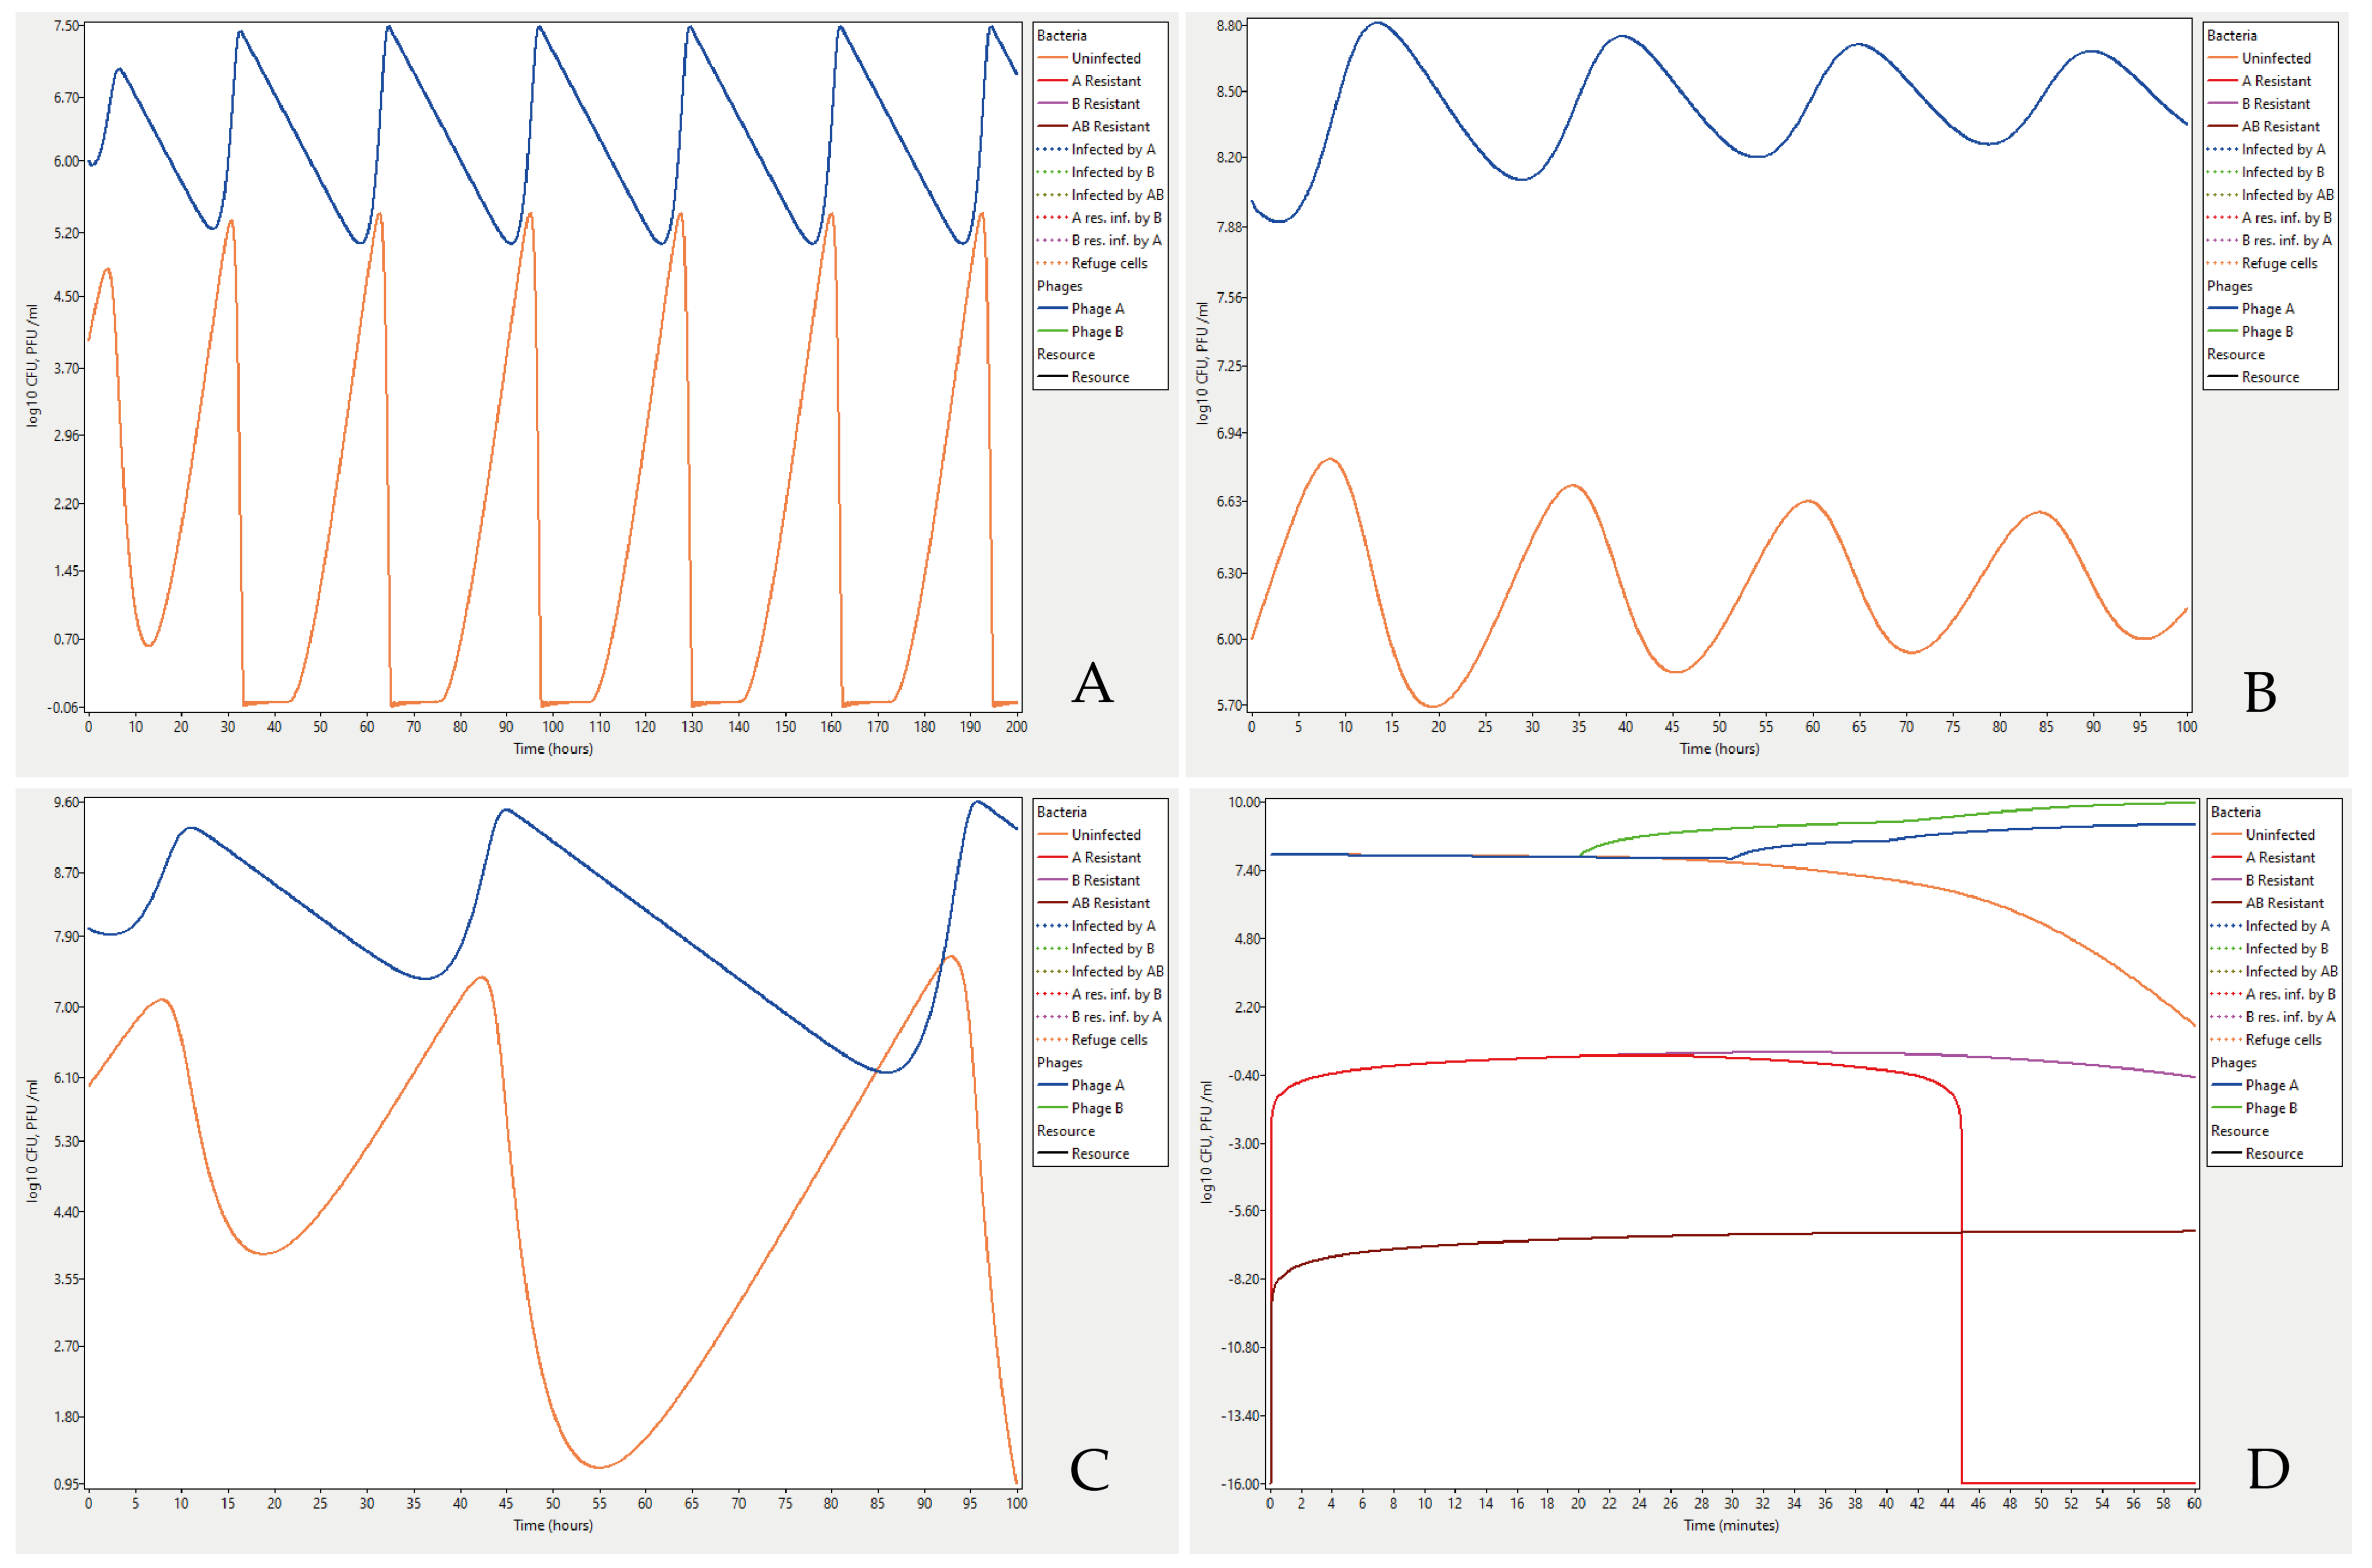
\includegraphics[width=\linewidth]{Plots/Sourced/cocktail_plot.png}
        \caption{
            Figure A) \textit{E. coli} infected with phage T4 in a chemostat exhibiting an oscillating growth behavior, following the model of \citet{bohannanEffectResourceEnrichment1997}. 
            Figure B) Oscillations of bacteria and phages can exist at higher titers, dependent on low resource concentration, following the model of \citet{lenskiDynamicsInteractionsBacteria1988}. 
            Figure C) As the concentration of resources change, this results in increasing oscillations, but not going extinct. 
            Figure D) A system modelling the interactions with phage A and B. 
        }
        \label{fig:sourced:cocktail_plot}
    \end{subfigure}
    \hfill
    \begin{subfigure}{0.49\linewidth}
        \centering
        \captionsetup{width=1\linewidth}
        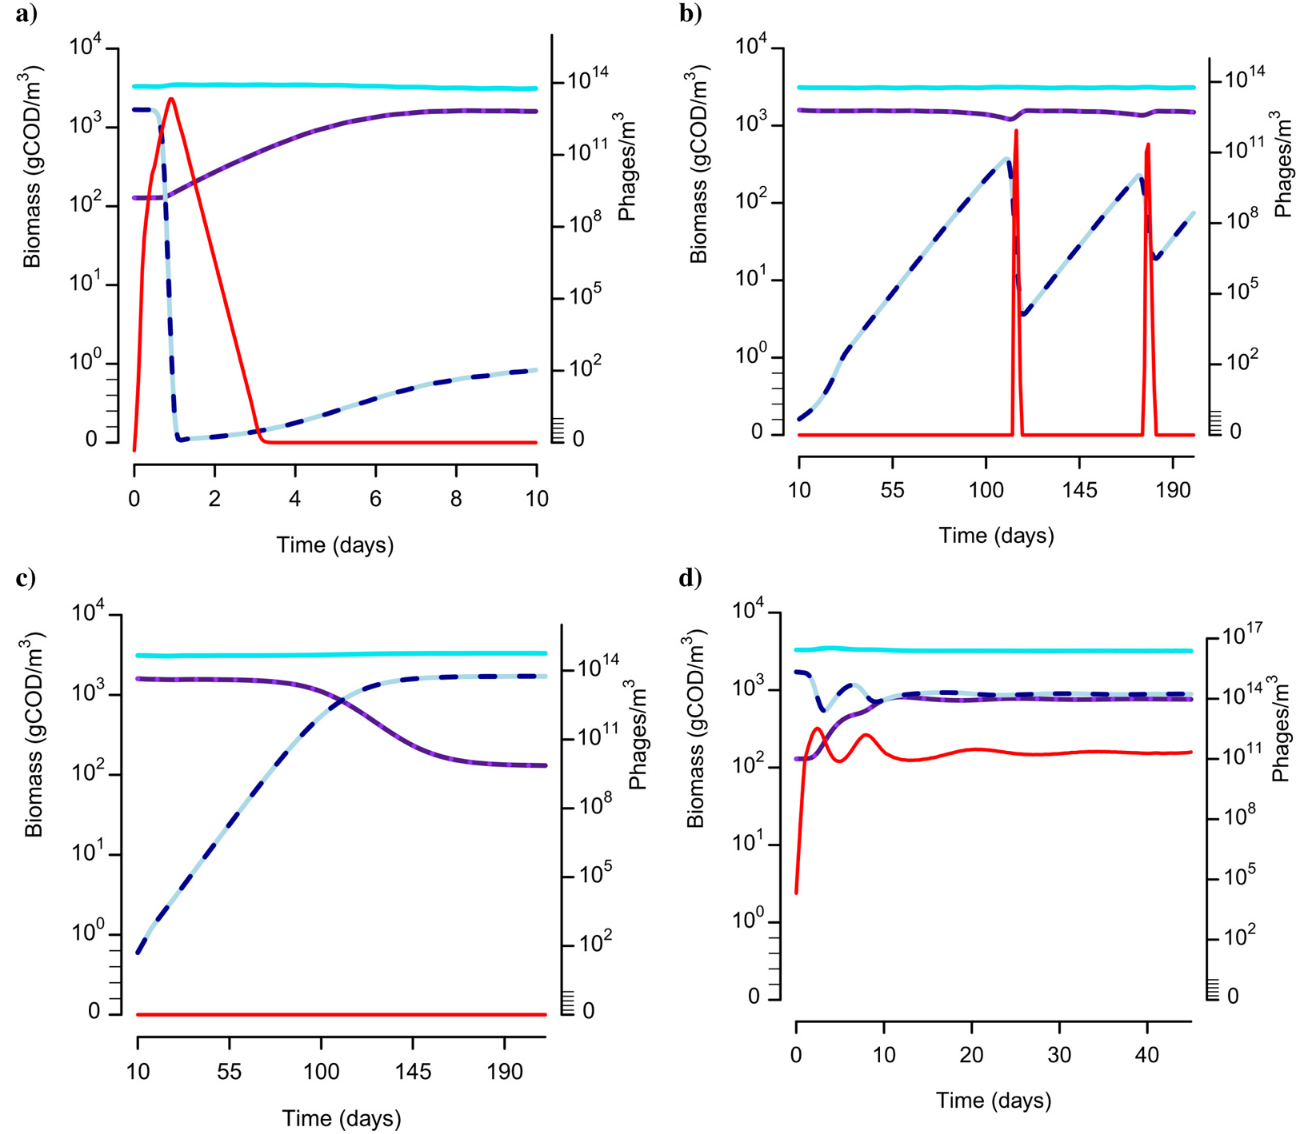
\includegraphics[width=\linewidth]{Plots/Sourced/phagedyn_plot.png}
        \caption{
            \textcolor[HTML]{551A8C}{\textbf{Purple}} is heterotrophic biomass, 
            \textcolor[HTML]{4580B4}{\textbf{Blue}} is foaming biomass, 
            \textcolor[HTML]{FF0000}{\textbf{Red}} is phages, 
            \textcolor[HTML]{01E6EE}{\textbf{Light Blue}} is total suspended solids. 
            Figure A) Biomass concentration immediately post phage dosing. 
            Figure B) Biomass concentration with low phage concentration and maintain low concentration post spike in population count. 
            Figure C) Biomass concentration when phages are extinct. 
            Figure D) Biomass concentration with a less virulent and low adsorption rate phage, co-existence with biomass reached. 
            A change in phage concentration shows a decrease in heterotrophic and foaming biomass \cite{krysiak-baltynSimulationPhageDynamics2017}. 
        }
        \label{fig:sourced:phagedyn_plot}
    \end{subfigure}
    \caption{Example output from Cocktail and PhageDyn respectively. For PhageDyn, concentration of heterotrophic biomass in an aerobic plug flow across four situations.
        See \citet{nilssonCocktailComputerProgram2022} and \citet{krysiak-baltynSimulationPhageDynamics2017} for more information on parameter values and supplementary resources. 
    }
    \label{fig:sourced:cocktail_and_phagedyn}
\end{figure}

\section{What Does Good Curve Behavior Look Like?}
A good bacteria growth curve looks like a mountain, with a clear rise, peak, and fall in bacteria levels. 
For a given IC, the bacteria start to consume resources and replicate leading to exponential growth. 
The phages infect the bacteria and eventually the bacteria lyse, releasing new phages. 
The new phages infect more bacteria, putting pressure on the bacteria growth. 
Eventually, more bacteria are being infected than being created, causing the decline in bacteria population. 
This decline can be quite sudden and quick. 

Both bacteria and phage population exhibit exponential growth. 
Similar to a classical predator-prey system, with the bacteria acting as the prey, and phages acting as the predator, the phage population lags behind the bacteria population.
The difference in peak bacteria and phage population times can be measured and quantified. 

If a bacteria colony starts at 100 bacteria, and grows at 4\% per minute, it will take about 112 minutes, or almost 2 hours for the colony to grow $100\times$. 
\begin{align}
    N &= Ae^rt \\ 
    10000 &= 100e^{0.04t} \\
    t &= frac{(ln(10000) - ln(100))}{0.04} \\
    t = 115.13
\end{align}

With pressure from phages, and potentially slower production rate while infected, the bacteria population might only increase $40\times - 80\times$, and have a slower growth rate. 